% rubber: module biber
\documentclass[xcolor=pst]{beamer}
\usepackage[utf8]{inputenc}
\usepackage{ngerman}
\usepackage{beamerthemesplit}
\usepackage{epsfig}
\usepackage{tikz}
\usepackage{siunitx}
\usepackage{pbox}
\usepackage{pdfpages}
\usepackage{verbatim}
\usepackage{units}
\usepackage{algpseudocode}

\usepackage{color}
\usetheme{Antibes}
%\usepackage{multirow}

% an seitenbreite angepasste tabellen
\usepackage{booktabs}
\usepackage{tabularx} % page-width
\usepackage{adjustbox}

% bibliographie
\usepackage[english]{cleveref}
\usepackage[style=numeric]{biblatex}
\addbibresource{literatur.bib}
\usepackage{appendixnumberbeamer}

\usetikzlibrary{shapes.geometric, calc, shapes}

% fusszeile so aufteilen, dass autoren und titel reinpassen und seitenzahl hinzu
\setbeamertemplate{footline}
{
  \leavevmode%
  \hbox{%
  \begin{beamercolorbox}[wd=.6\paperwidth,ht=2.25ex,dp=1ex,center]{author in head/foot}%
    \usebeamerfont{author in head/foot}\insertshortauthor
  \end{beamercolorbox}%
  \begin{beamercolorbox}[wd=.4\paperwidth,ht=2.25ex,dp=1ex,center]{title in head/foot}%
    \usebeamerfont{title in head/foot}\insertshorttitle\hspace*{2.5em}\insertframenumber
  \end{beamercolorbox}}%
  \vskip0pt%
}

% keine navigationssymbole in der fusszeile
\beamertemplatenavigationsymbolsempty

% so definiert man neue makros
\newcommand{\IFF}{\Leftrightarrow}
\newcommand{\todo}[1]{\textbf{\color{red}todo:\color{black}#1}}

\author{
  Lukas Götz, Stefan Dang \& Dorle Osterode
}
\title{Gt-Scaffolder: TODO}
\institute[FBI - UniHH]{Universität Hamburg - Fachbereich Bioinformatik}
\date{2015-01-30}

\subject{}
\keywords{}

\begin{document}
\begin{frame}[plain]
  \titlepage
\end{frame}

% keine seitenzahl auf der inhaltsangabe zeigen (theme nur fuer diese folie anpassen)
\bgroup
\makeatletter
\setbeamertemplate{footline}
{
  \leavevmode%
  \hbox{%
  \begin{beamercolorbox}[wd=.6\paperwidth,ht=2.25ex,dp=1ex,center]{author in head/foot}%
    \usebeamerfont{author in head/foot}\insertshortauthor
  \end{beamercolorbox}%
  \begin{beamercolorbox}[wd=.4\paperwidth,ht=2.25ex,dp=1ex,center]{title in head/foot}%
    \usebeamerfont{title in head/foot}\insertshorttitle\hspace*{2.5em}
  \end{beamercolorbox}}%
  \vskip0pt%
}
\makeatother
\begin{frame}{Übersicht}
  \tableofcontents
\end{frame}
\egroup % ab hier das normale theme weiterverwenden


\section{Motivation}
\subsection{Scaffolding}
\begin{frame}
\setcounter{framenumber}{1}
  \frametitle{Einführung}

  \begin{columns}
    \begin{column}{.45\textwidth}
      \begin{itemize}
      \item Assemblierung $\rightarrow$ Mehrere unabhängige Contigs
      \begin{itemize}
        \item Ungleichmäßige Coverage
        \item Wiederholungen
      \end{itemize}
      \item Motivation: Einordnung der Contigs in Scaffolds
      \begin{itemize}
        \item Richtung und relative Anordnung
        \item Paarweiser Abstand
      \end{itemize}
      \end{itemize}
    \end{column}
    \begin{column}{.45\textwidth}
      \begin{center}
        \begin{figure}[t]
          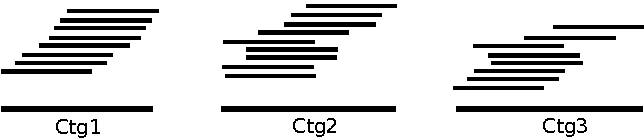
\includegraphics[width=\textwidth,height=0.8\textheight,keepaspectratio]{figures/Scaffolding.pdf}
        \end{figure}
        \vspace{.75cm}
        \begin{figure}[t]
          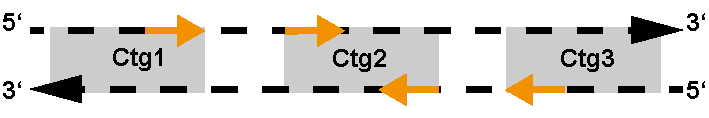
\includegraphics[width=\textwidth,height=0.8\textheight,keepaspectratio]{figures/Scaffolding_2.pdf}
        \end{figure}
      \end{center}
    \end{column}
  \end{columns}
  \let\thefootnote\relax\footnotetext{\cite{Pop:2009dp}}
\end{frame}

\begin{frame}
  \frametitle{Einführung}
  \begin{itemize}
  \item Verwendung der Read-Paar Informationen:
    \begin{itemize}
    \item Fragmentgröße
    \item Position auf Contigs
    \end{itemize}
  \item Read-Paare stammen aus paired-end oder mate-pair Sequenzierung
  \end{itemize}
\end{frame}

\begin{frame}
  \frametitle{Scaffolding Problem}
  \begin{center}
    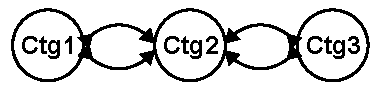
\includegraphics[width=0.5\textwidth,height=0.8\textheight,keepaspectratio]{figures/Scaffolding_3.pdf}
  \end{center}
  \begin{itemize}
  \item Scaffold Graph:
    \begin{itemize}
    \item Knoten entsprechen Contigs
    \item Kanten beschreiben Read-Paar
      Informationen
    \item bidirektionaler Graph
    \end{itemize}
  \item Scaffolding ist NP-vollständig
  \item Strategie: Zerlegung in
    Teilprobleme, die unabhängig voneinander gelöst werden
  %% \item Beschreibung des Scaffolding Problems mit Hilfe eines
  %%   Graphen (Scaffold Graph), wobei deren Zusammenhangskomponenten
  %%   Teilprobleme darstellen
  \end{itemize}
  \let\thefootnote\relax\footnotetext{\cite{Huson:2002kf}}
\end{frame}

\subsection{Motivation}
\begin{frame}
  \frametitle{Motivation}
  \begin{itemize}
  \item Ziel: Entwicklung einer Scaffolding-Software
  \begin{itemize}
    \item Aufbauend auf Assemblierungs-Software \textit{Readjoiner} (\textit{GenomeTools})
  \end{itemize}
  \item Methodische Anlehnung an \textit{String Graph Assembler}
  \begin{itemize}
    \item Vereinfachung und Partitionierung eines Scaffold-Graphen
    \item Berechnung des Scaffolds als Pfad mit max. Sequenzabdeckung
  \end{itemize}
  \end{itemize}
  \let\thefootnote\relax\footnotetext{\cite{Gonnella:2012gn,Simpson:2012ef}}
\end{frame}

\section{Methoden}
% \begin{frame}
%   \frametitle{Allgemein}
%   \begin{itemize}
%   \item Reimplementation der Scaffolding Methode von SGA (C++) im
%     Rahmen von Genometools (C)
%   \item basiert auf Konstruktion eines Graphen über die Beziehungen
%     zwischen Contigs (Scaffold Graph)
%   \end{itemize}
% \end{frame}

\begin{frame}
  \frametitle{Gt-Scaffolder}
  \begin{itemize}
  \item Eingabe:
    \begin{itemize}
    \item Contigs
    \item Distanzinformationen
    \item A-Statistik %spelling?
    \end{itemize}
  \item Ausgabe:
    \begin{itemize}
    \item Scaffolds
    \item (rekonstruierte Sequenzen)
    \end{itemize}
  \end{itemize}
\end{frame}

\begin{frame}
  \frametitle{Übersicht der Schritte}
  \begin{itemize}
  \item Konstruktion des Scaffold Graph:
    \begin{itemize}
    \item nicht-repetitive Contigs als Knoten
    \item bidirektionalen Kanten zwischen Contigs
    \end{itemize}
  \item Filterung des Graphen:
    \begin{itemize}
    \item inkonsistente Kanten
    \item polymorphe Knoten
    \item Zyklen
    \end{itemize}
  \item Ermittlung aller Zusammenhangskomponenten
  \item Bestimmung des Pfades mit größter Sequenzabdeckung für jede
    Zusammenhangskomponente
  \end{itemize}
  TODO:\ Illustrieren der einzelnen Schritte
\end{frame}

\section{Ergebnisse}

\begin{frame}
  \frametitle{Vergleichender Scaffold mit SGA:\ Ergebnisse}
  \begin{itemize}
    \item Daten: Referenzsequenzen
    \begin{itemize}
      \item S. cerevisiae (12Mbp, Ensemble R64\-1\-1)
      \item C. elegans (100Mbp, Ensemble WBcel235)
    \end{itemize}
    \item Simulierte Paired-End-Reads durch \textit{art\_illumina}
    \begin{itemize}
      \item Read-Länge 150 bp
      \item Coverage 20
      \item Fragmentlänge 400 bp
      \item Standardabweichung 10 bp
    \end{itemize}
    \item Vergleich des Scaffolding-Schrittes
    \begin{itemize}
      \item Assemblierung der Reads durch SGA-E.coli-Beispielpipeline
      \item TODO:\ Hardware einfügen (CPU, RAM, OS, bit)
    \end{itemize}
  \end{itemize}
  \let\thefootnote\relax\footnotetext{\cite{Earl:2011gt,Huang:2012kq}}
\end{frame}



\begin{frame}
  \frametitle{Vergleichender Scaffold mit SGA:\ Ergebnisse}
  \begin{table}
      \adjustbox{max height=\dimexpr\textheight-5.5cm\relax, max width=\textwidth}{
      \begin{tabular}{cccccc}
          \toprule
          Program name & Total span (Mbp) & \#Scaffolds & $N50$   & CPU (min) & Mem (kB) \\
          \midrule
          SGA          & 11.08            &       600   & 32276   & 1.95   &  29568 \\
          Gt Scaffold  & 0000             &       600   & 0000.00 & 2.44   &  12892 \\
          \bottomrule
      \end{tabular}}
      \caption{S. cerevisiae}
  \end{table}

  \begin{table}
      \adjustbox{max height=\dimexpr\textheight-5.5cm\relax, max width=\textwidth}{
      \begin{tabular}{cccccc}
          \toprule
          Program name & Total size (kb) & \#Scaffolds & $N50$   & CPU (min) & Mem (GB) \\
          \midrule
          SGA          & 0000            &             & 0000.00 & 0.0       & 00.0 \\
          Gt Scaffold  & 0000            &             & 0000.00 & 0.0       & 00.0 \\
          \bottomrule
      \end{tabular}}
      \caption{C. elegans}
  \end{table}
\end{frame}

\section{Diskussion und Ausblick}
\begin{frame}
  \frametitle{Diskussion}
  \begin{itemize}
  \item Gründe für neue Implementation
    \begin{itemize}
    \item geringerer Speicherplatzverbrauch, schnellere Laufzeit
       für Gt-Scaffolder (C-Implementation) im Vergleich zu
       SGA-Scaffolder (C++ Implementation) bei gleicher Güte
       der Ergebnisse (quod esset demonstrandum)
    \item Keine externen Software-Abhängigkeiten:
      %% , Einbau von
      %% Abyss DistEst in Gt-Scaffolder (zur Ermittlung der Read-Paar
      %% Informationen) und Berechnung der A-Statistik durch Read-Joiner
      %% anstelle von Pysam
    \end{itemize}
  \end{itemize}
  \begin{tikzpicture}[node distance=.75cm]
    \tikzstyle{prog}=[draw, rectangle, rounded corners, font=\tiny, rotate=90];
    \node[prog] (prep) {preprocess};
    \node[prog, below of=prep] (index) {index};
    \node[prog, below of=index] (correct) {correct};
    \node[prog, below of=correct] (index2) {index};
    \node[prog, below of=index2] (filter) {filter};
    \node[prog, below of=filter] (overlap) {overlap};
    \node[prog, below of=overlap] (assemble) {assemble};
    \node[prog, below of=assemble, fill=red!40] (bindex) {index};
    \node[prog, below of=bindex, fill=red!40] (aln) {align};
    \node[prog, below of=aln, fill=red!40] (sampe) {sampe};
    \node[prog, below of=sampe, rectangle split, rectangle split parts=3, yshift=-.45cm, rectangle split part fill={blue!40, green!40, blue!40}] (bam2de) {\nodepart{one}fixmate\nodepart{two}samtools\nodepart{three}DistanceEst};
    \node[prog, below of=bam2de, yshift=-.45cm, fill=yellow!40] (pysam) {astat};
    \node[prog, below of=pysam] (scaff) {scaffold};
    \node[prog, below of=scaff] (scaf2fasta) {scaf2fasta};

    \path[->]
    (prep) edge (index)
    (index) edge (correct)
    (correct) edge (index2)
    (index2) edge (filter)
    (filter) edge (overlap)
    (overlap) edge (assemble)
    (assemble) edge (bindex)
    (bindex) edge (aln)
    (aln) edge (sampe)
    (sampe) edge (bam2de)
    (bam2de) edge (pysam)
    (pysam) edge (scaff)
    (scaff) edge (scaf2fasta);
  \end{tikzpicture}

  \begin{tikzpicture}[node distance=.75cm]
    \tikzstyle{prog}=[draw, rectangle, rounded corners, font=\tiny, rotate=90];
    \node[prog] (prefilter) {prefilter};
    \node[prog, below of=prefilter] (overlap) {overlap};
    \node[prog, below of=overlap] (assembly) {assembly};
    \node[prog, below of=assembly] (scaffold) {scaffold};

    \path[->]
    (prefilter) edge (overlap)
    (overlap) edge (assembly)
    (assembly) edge (scaffold);
  \end{tikzpicture}
\end{frame}

\begin{frame}
  \frametitle{Ausblick}
  \begin{itemize}
  \item was wir noch alles machen muessen (kann erst am ende
    ausgefuellt werden)
  \end{itemize}
\end{frame}


\appendix
\section*{Bibliographie}
\begin{frame}{Bibliographie}
    %\nocite{Hernandez:2014jp, Hernandez:2008jw}
    \printbibliography
\end{frame}
\end{document}
